\graphicspath{{chapters/18/images}}
\chapter{Free energy calculations}

\section{Free energy perturbation theory}
Two states $A$ and $B$:

$$U_A(\vec{r}_1, \dots, \vec{r}_n)\land U_{B}(\vec{r}_1, \dots, \vec{r}_N)$$

$$\Delta A_{AB} = -kT\ln Q_B + kT\ln Q_A = -kT\ln\frac{Z_B}{Z_A}$$

$$Z_A = \int d^N\vec{r}e^{-\beta U_A(\vec{r}_1, \dots, \vec{r}_N)}\qquad Z_B = \int d^N\vec{r}e^{-\beta U_B(\vec{r}_1, \dots, \vec{r}_N)}$$

Difficult to compute.

$$Z_B = \int d^N\vec{r}e^{-\beta U_B(\vec{r}_1, \dots, \vec{r}_N)} = \int d^N\vec{r}e^{-\beta[U_B(\vec{r}_1, \dots, \vec{r}_N)-U_{A}(\vec{r}_1, \dots, \vec{r}_N)]}e^{-\beta U_A(\vec{r}_1, \dots, \vec{r}_N)}$$

$$\frac{Z_B}{Z_A} = \frac{1}{Z_A}\int d^N\vec{r}e^{-\beta[U_B(\vec{r}_1, \dots, \vec{r}_N)-U_{A}(\vec{r}_1, \dots, \vec{r}_N)]}e^{-\beta U_A(\vec{r}_1, \dots, \vec{r}_N)}$$


$$\Delta A_{AB} = -kT\ln\frac{Z_B}{Z_A}\qquad\frac{Z_B}{Z_A} = \biggl\langle e^{-\beta[U_B(\vec{r}_1, \dots, \vec{r}_N)-U_A(\vec{r}_1, \dots, \vec{r}_N)]}\biggr\rangle_A$$

Free energy perturbation formula:

$$\Delta A_{AB} = -kT\ln\biggl\langle e^{-\beta[U_B(\vec{r}_1, \dots, \vec{r}_N)-U_A(\vec{r}_1, \dots, \vec{r}_N)]}\biggr\rangle_A$$

In case of poor overlap:

$$\Delta A_{AB}=0kT\sum\limits_{\alpha=1}^{M-1}\ln\bigl\langle e^{-\beta\Delta U_{\alpha, \alpha+1}(\vec{r}_1, \dots,\vec{r})N}\bigr\rangle_\alpha$$

	\subsection{Adiabatic switching}

	$$U(\vec{r}_1, \dots, \vec{r}_N, \lambda) \equiv f(\lambda)U_A(\vec{r}_1, \dots, \vec{r}_N)+g(\lambda)U_B(\vec{r}_1, \dots, \vec{r}_N)$$

	$$f(0) = 1, \quad f(1) = 0,\quad g(0) = 0, \quad g(1) = 1$$

	$$Q(N, V, T, \lambda) = C_N\int d^N\vec{p}d^N\vec{r}e^{-\beta\biggl[\sum\limits_{i=1}^N\frac{\vec{p}_o^2}{2m_i}+U(\vec{r}_1, \dots, \vec{r}_N, \lambda)\biggr]}$$

	$$A(N, V, T, \lambda) = -kT\ln Q(N, V, T, \lambda)$$

	$$\frac{\partial A}{\partial \lambda} = -\frac{kT}{Q}\frac{\partial Q}{\partial \lambda} = -\frac{kT}{Z}\frac{\partial Z}{\partial\lambda}$$

	$$\frac{kT}{Z}\frac{\partial Z}{\partial \lambda} = \frac{kT}{Z}\frac{\partial}{\partial\lambda}\int d^N\vec{r}e^{-\beta U(\vec{r}_1, \dots, \vec{r}_N, \lambda)} = \frac{kT}{Z}\int d^{N}\vec{r}\biggl(-\beta\frac{\partial U}{\partial\lambda}\biggr)e^{-\beta U(\vec{r}_1, \dots, \vec{r}_N)} = -\biggl\langle\frac{\partial U}{\partial\lambda}\biggr\rangle$$

	\subsection{Thermodynamics integration}

	$$\Delta A_{AB} = \int_0^1\biggl(\frac{\partial A}{\partial \lambda}\biggr)d\lambda = \int_0^1\biggl\langle\frac{\partial U}{\partial\lambda}\biggr\rangle_\lambda d\lambda$$

	The aim is to make the region between $\lambda=0$ and $\lambda=1$ energetically unfavourable.

	$$\mathcal{H}_\lambda(\vec{r}, \lambda, \vec{p}, p_\lambda) = \frac{p_\lambda^2}{2m_\lambda} + \sum\limits_{i=1}^N\frac{\vec{p}_i^2}{2m_i} + U(\vec{r}_1, \dots, \vec{r}_N, \lambda)$$

	$$Q(N, V, T) = \int dp_\lambda\int d^N\vec{p}\int_0^1d\lambda\int d^N\vec{r}e^{-\beta\mathcal{H}_\lambda(\vec{r},\lambda,\vec{p}, p_\lambda)}$$

	Probability distribution $P(\lambda') = \langle\delta(\lambda-\lambda')\rangle$.
	Free energy profile: $A(\lambda') = -kT\ln P(\lambda')$.

	$$A(1) = A(0) = -kT\ln\frac{P(1)}{P(0)} = -kT\ln\frac{Q_B}{Q_A} = \Delta A_{AB}$$


	\subsection{Adiabatic free energy dynamics}

	\begin{figure}[H]
		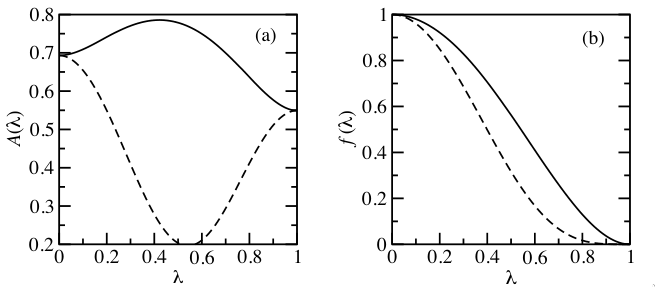
\includegraphics[width=\textwidth]{adiabatic-free-energy-dynamics}
		\caption{Adiabatic free energy dynamics}
		\label{fig:adiabatic-free-energy-dynamics}
	\end{figure}

	Probability to cross a barrier $U^{\ddagger}$ is proportional to $e^{-\frac{U^{\ddagger}}{kT}}$.
	Raise the temperature of teh $\lambda$ degree of freedom: $\biggl\langle\frac{p_\lambda^2}{2m_\lambda}\biggr\rangle = kT_\lambda$.
	Adiabatic decoupling: increases $m_\lambda$ until the $\lambda$ degree of freedom is decoupled from all other degrees of freedom: $\lambda$ is almost fixed:

	$$Z(\lambda, \beta) = \int d^N\vec{r}e^{-\beta U(\vec{r}, \lambda)}\qquad\text{ Correct if }\lambda\text{ is fixed}$$

	Potential of mean force in $\lambda:-\frac{1}{\beta}\ln Z(\lambda, \beta)$.
	$\lambda$ moves quasi-independently from the physical degrees of freedom in the potential of mean force, subject to an effective Hamiltonian:

	$$\mathcal{H}_{eff}(\lambda, p_\lambda) = \frac{p_\lambda^2}{2m_\lambda} -\frac{1}{\beta}\ln Z(\lambda, \beta)$$

	$\lambda$ is thermostatted at a temperature $T_\lambda>T$, hence the obtained canonical distribution is:

	$$P_{adb}(\lambda, p_\lambda, \beta, \beta_\lambda)\propto e^{-\beta_\lambda\mathcal{H}_{eff}(\lambda, p_\lambda)}$$

	$$\tilde{P}_{adb}(\lambda, \beta, \beta_\lambda) = \int dp_\lambda P_{adb}(\lambda, p_\lambda, \beta, \beta_\lambda)\propto e^{\beta_\lambda\ln \frac{Z(\lambda, \beta)}{\beta}} = [Z(\lambda, \beta)]^{\frac{\beta_\lambda}{\beta}}$$

	$$A(\lambda) = -kT_\lambda\ln\tilde{P}_{adb}(\lambda, \beta, \beta_\lambda) = -kT\ln Z(\lambda, \beta) + const$$

\section{Jarzynski's equality}
Work-free energy inequality: $W_{AB}\ge \Delta A_{AB}$.
$W_{AB}$ is a thermodynamic quantity and can be expressed as a thermodynamic average:

$$W_{AB} = \langle\mathcal{W}_{AB}(x)\rangle$$

Initial distribution of microstates $x_0\in A$.
The work $\mathcal{W}_{AB}(x_0)$ is a functional of the path $\mathcal{W}_{AB}[x_t] = \mathcal{W}_{AB}[x_t(x_0)] = \mathcal{W}_{AB}(x_0)$.

$$W_{AB} = \langle\mathcal{W}_{AB}(x_0)\rangle_A=\frac{C_N}{Q_A(N, V, T)}\int dx_0e^{-\beta\mathcal{H}_A(x_0)}\mathcal{W}_{AB}(x_0)\ge \Delta A_{AB}$$

Jarzynski:

$$\langle e^{-\beta\mathcal{W}_{AB}(x_0)}\rangle_A = \frac{C_N}{Q_A(N, V, T)}\int dx_0e^{-\beta\mathcal{H}_A(x_0)}e^{-\beta\mathcal{W}_{AB}(x_0)} = e^{-\beta\Delta A_{AB}}$$

$$\Delta A_{AB} = -kT\ln\langle e^{-\beta\mathcal{W}_{AB}(x_0)}\rangle_A$$

Time dependent Hamiltonian: $\mathcal{H}(\vec{r}, \vec{p}, t) = \sum\limits_{i=1}^N\frac{\vec{p}_i^2}{2m_i} + U(\vec{r}, t)$.

$$\frac{d\mathcal{H}}{dt} = \nabla_{x_t}\mathcal{H}\cdot\dot{x_t}+\frac{\partial\mathcal{H}}{\partial t}$$

$$\int_0^\tau\frac{d\mathcal{H}}{dt} = \underbrace{\int_0^\tau\nabla_{x_t}\mathcal{H}\cdot\dot{x}_tdt}_{\text{Heat}}+\underbrace{\int_0^\tau\frac{\partial\mathcal{H}}{\partial t}dt}_{\text{Work}}$$

$$\mathcal{W}_{t'}(x_0) = \int_0^{t'}\frac{\partial\mathcal{H}(x_t(x_0), t)}{\partial t}dt\qquad \mathcal{W}_{AB}(x_0) = \mathcal{W}_\tau(x_0)$$

Hamilton's equations: $\nabla_{x_t}\mathcal{H}\cdot\dot{x}_t = 0\Rightarrow\frac{\partial\mathcal{H}}{\partial t} = \frac{d\mathcal{H}}{dt}$

$$W_{t'}(x_0) = \int_0^{t'}\frac{\partial\mathcal{H}(x_t(x_0),t)}{\partial t}dt = \int_0^{t'}\frac{d\mathcal{H}(x_t(x_0), t)}{dt}dt = \mathcal{H}(x_{t'}(x_0), t') - \mathcal{H}(x_0, 0)$$

$$\mathcal{W}_{AB}(x_0) = \mathcal{W}_\tau(x_0) = \mathcal{H}(x_\tau(x_0), \tau)-\mathcal{H}(x_0,0)\qquad \mathcal{H}(x_0, 0) = \mathcal{H}_A(x_0)$$

Hence:

$$\langle e^{-\beta\mathcal{W}_{AB}}\rangle_A = \frac{C_N}{Q_A(N, V, T)}\int dx_0e^{-\beta\mathcal{H}_A(x_0)}e^{-\beta[\mathcal{H}(x_\tau(x_0), \tau)-\mathcal{H}_A(x_0)]} = \frac{C_N}{Q_A(N, V, T)}\int dx_0e^{-\beta\mathcal{H}(x_\tau(x_0), \tau)}$$

Change of coordinates from $x_0$  to $x_\tau(x_0)$.
By Liouville's theorem $dx_\tau = dx_0$:

$$\langle e^{-\beta\mathcal{W}_{AB}}\rangle_A = \frac{C_N}{Q_A(N, V, T)}\int dx_\tau e^{-\beta\mathcal{H}_B(x_\tau)} = \frac{Q_B(N, V, T)}{Q_A(N, V, T)} = e^{-\beta\Delta A_{AB}}$$

Other versions of this proof are available, with thermostats for instance.
Application: pulling experiments.
A time-dependent potential drives the end-to-end distance $|\vec{r}_1-\vec{r}_N|$ of a peptide away form its equilibrium value in the folded state:

$$U(\vec{r}_1, \dots, \vec{r}_N, t) = U_o(\vec{r}_1, \dots, \vec{r}_N) + \frac{1}{2}k\bigl(|\vec{r}_1-\vec{r}_N|-r_{eq}-vt\bigr)^2$$

Ensemble of initial conditions with different pulling rates.

$$\langle e^{-\beta\mathcal{W}_{AB}}\rangle_A = e^{-\beta\Delta A_{AB}}$$

Problems: work values have a distribution $P(\mathcal{W}_\tau)$.

$$\langle e^{-\beta\mathcal{W}_\tau}\rangle= \int\mathcal{W}_\tau P(\mathcal{W}_\tau)e^{-\beta\mathcal{W}_\tau}$$

If and only if $P(\mathcal{W}_\tau)$ is Gaussian:

$$\ln\langle e^{-\beta\mathcal{W}_\tau}\rangle\simeq-\beta\langle\mathcal{W}_\tau\rangle + \frac{\beta^2}{2}(\langle\mathcal{W}_\tau^2\rangle-\langle\mathcal{W}_\tau\rangle^2)$$

The final state is not at equilibrium if the driving force is too strong.

\section{Replica exchange Monte Carlo}
$M$ independent copies of a system: each replica is assigned a different value of some physical control variable or parameter.

	\subsection{Parallel tempering}
	$M$ independent copies of a system: $T_M>T_{M-1}>T_{M-2}>\cdots>T_1$, where $T_1$ is the temperature of the canonical distribution to be sampled.
	Configuration of replicas $\vec{r}^{(1)}, \dots, \vec{r}^{(M)}$.
	Independent replicas: total probability distribution:

	$$F(\vec{r}^{(1)}, \dots, \vec{r}^{(M)}) = \prod\limits_{K=1}^Mf_K(\vec{r}^{(K)})\qquad f_K(\vec{r}^{(K)}) = \frac{e^{-\beta_K U(\vec{r}^{(K)})}}{Q(N ,V, T_K)}$$

	Select randomly two neighbouring replicas and attempt replica exchange:

	$$(\vec{r}^{(K)}, \vec{r}^{(K+1)})\rightarrow (\tilde{\vec{r}}^{(K)}, \tilde{\vec{r}}^{(K+1)})\qquad\text{ with }\qquad \tilde{\vec{k}}^{(K+1)} = \vec{r}^{(K)}\land \tilde{\vec{r}}^{(K+1)}=\vec{r}^{(K)}$$

	Coordinates are merely exchanged:

	$$T(\tilde{\vec{r}}^{(K)}, \tilde{\vec{r}}^{(K+1)}|\vec{r}^{(K)}, \vec{r}^{(K+1)}) = T(\vec{r}^{(K)}, \vec{r}^{(K+1)}|\tilde{\vec{r}}^{(K)}, \tilde{\vec{r}}^{(K+1)})$$

	Acceptance probability:

	$$A(\tilde{\vec{r}}^{(K)}, \tilde{\vec{r}}^{(K+1)}|\vec{r}^{(K)}, \vec{r}^{(K+1)}) = A(\vec{r}^{(K+1)}, \vec{r}^{(K)} | \vec{r}^{(K)}, \vec{r}^{(K+1)})$$

	$$A(\vec{r}^{(K+1)}, \vec{r}^{(K)} | \vec{r}^{(K)}, \vec{r}^{(K+1)}) = \min\biggl[1, \frac{f_K(\vec{r}^{(K+1)})f_{K+1}*\vec{r}^{(K)}}{f_K(\vec{r}^{(K)})f_{K+1}(\vec{r}^{(K+1)})}\biggr] = \min[1, e^{-\Delta_{K, K+1}}]$$

	$$\Delta_{K, K+1} = (\beta_k-\beta_{K+1})[U(\vec{r}^{(K+1)}) - U(\vec{r}^{(K)})]$$

	\subsection{Wang-Landau sampling}

	$$Q(N, V, T) = \frac{1}{E_0}\int_0^{\infty}dEe^{-\beta E}\Omega(N, V, E)\Rightarrow Q(\beta) = \int_0^{\infty}dEe^{-\beta E}\Omega(E)$$

	Now $\Omega(E)$< the inverse of the probability of state $E$ is computed directly.
	Assign $\Omega(E)=1\forall E$ discredited.
	Trial move: $E_1\rightarrow E_2$:

	$$A(E_2|E_1) = \min\biggl[1, \frac{\Omega(E_1)}{\Omega(E_2)}\biggr]$$

	After each move: $\Omega(E)\rightarrow \Omega(E)f\quad f>1$.
	Histogram $h(E)$ of visited states.
	Once $h(E)$ is flat enough a new value $f_{new} = \sqrt{f_{old}}$ is switched and the algorithms continue until convergence.
	There is no detailed balance due to $f$.
